\documentclass[../main.tex]{subfiles}

\makeatletter
\@ifundefined{fromRoot}{%
  \newcommand{\fromRoot}[1]{../#1}
  
  \usepackage{xr}
  \externaldocument{../main}
}{}

\def\input@path{{\subfix{../}}}
%or: \def\input@path{{/path/to/folder/}{/path/to/other/folder/}}
\makeatother

\graphicspath{{\subfix{../}}}

\hypersetup{
    pdfauthor   = {Camille MONIÈRE},
    pdftitle    = {Th\`{e}se (Présentation: contexte)},
    pdfsubject  = {Th\`{e}se (Présentation: contexte)},
%    pdfkeywords = {mots-cl\'{e}s},
}

\begin{document}

\section{Introduction}

\subsection{Contexte}

\begin{frame}{Du contexte}
  \begin{overlayarea}{\linewidth}{.2\textheight}
    Coucou
  \end{overlayarea}
  
  \begin{columns}
    \begin{column}{.3\linewidth}
      \hfill
    \end{column}
    \begin{column}{.6\linewidth} \centering
      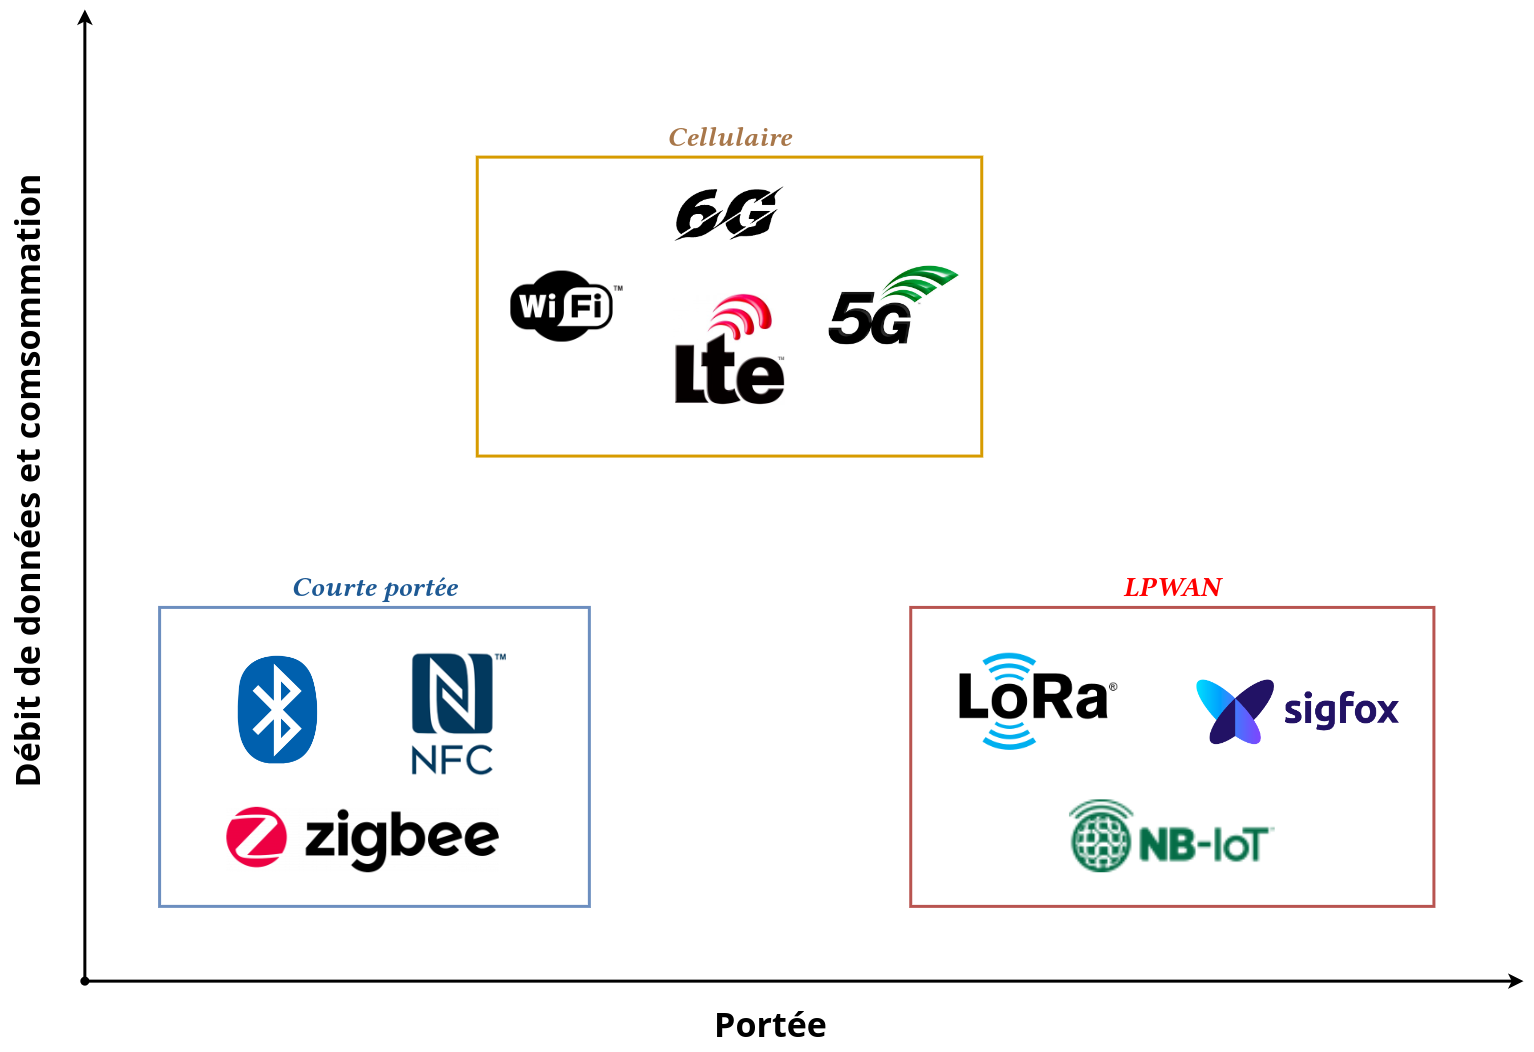
\includegraphics[width=\linewidth]{figures/drawiopdf/lpwan_and_co}
    \end{column}
    \begin{column}{.1\linewidth}
      \hfill
    \end{column}
  \end{columns}
\end{frame}

\subsection{Le projet \acrfull{qcsp}}

\begin{frame}{}
  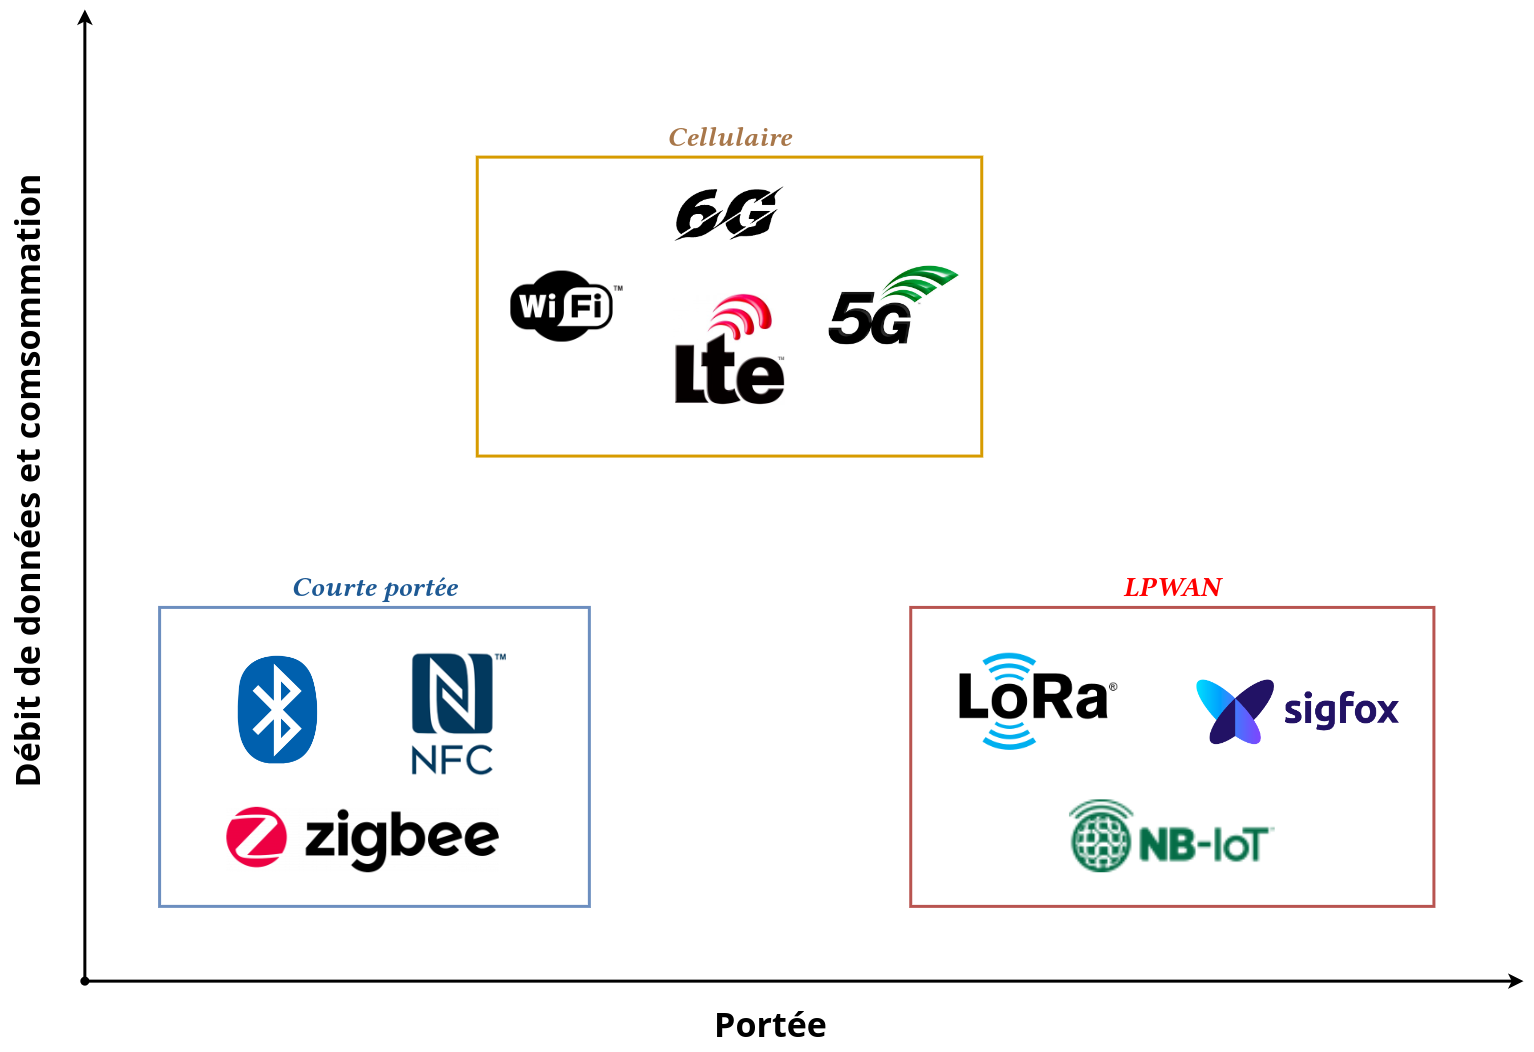
\includegraphics[width=0.9\linewidth]{figures/drawiopdf/lpwan_and_co}
\end{frame}

\end{document}
